\documentclass[11pt]{article}
\usepackage[T1]{fontenc}
\usepackage{times}%, babel}
\usepackage{secdot,natbib}
\usepackage{latexsym, amsthm, amsmath, amssymb, color, rotating, multirow, graphicx, hhline, array, tablefootnote}
\usepackage{scalefnt, enumerate}
\usepackage{footnote}
\usepackage{threeparttable,booktabs}
\usepackage{natbib}
\usepackage[hyphens]{url}
%\usepackage{bm, url}
%\usepackage{slashbox}
\usepackage{tikz,pgfplots}
\usepackage{lscape}
%\usepackage{subcaption}
\usepackage[margin=10pt,font=small,labelfont=bf,labelsep=endash]{caption}
\usepackage{subfigure}
\usepackage{tabularx}
\usepackage{booktabs}

\usepackage{kotex} %Korean TeX
%\usepackage[latin9]{inputenc} % kotex package와 충돌. 향후 kotex 삭제하면 될 듯.




%%% ----------------------------------------------------------------------
%\clubpenalty=10000 \widowpenalty=10000
%\renewcommand{\baselinestretch}{1.5}
% \renewcommand{\theequation}{{\rm \thesection.\arabic{equation}}}
\renewcommand{\theequation}{{\rm \arabic{equation}}}
\oddsidemargin 0in  %.10in
\evensidemargin 0in
\hyphenpenalty 2000

\textwidth 6.5in    %6.5
\textheight 8.75in     %8.5
\topmargin 0.0in      %0in
\headsep 0in \makeatletter
\newcommand{\singlespacing}{\let\CS=\@currsize\renewcommand{\baselinestretch}{1.1}\tiny\CS}
\newcommand{\doublespacing}{\let\CS=\@currsize\renewcommand{\baselinestretch}{1.5}\tiny\CS}
\newcommand{\realdoublespacing}{\let\CS=\@currsize\renewcommand{\baselinestretch}{2.0}\tiny\CS}
\newcommand{\mydoublespacing}{\let\CS=\@currsize\renewcommand{\baselinestretch}{1.499}\tiny\CS}

\newtheorem{theorem}{Theorem}[section]
\newtheorem{proposition}[theorem]{Proposition}
\newtheorem{lemma}[theorem]{Lemma}
\newtheorem{corollary}[theorem]{Corollary}

\def\N{\mathbb{N}}
\def\1{\mathbf{1}}
\def\P{\mathbf{P}}
\def\E{\mathbf{E}}
\newcommand{\maximize}{\mathop{\mbox{{\rm maximize}}}\limits}
\newcommand{\minimize}{\mathop{\mbox{{\rm minimize}}}\limits}
\newcommand{\argmax}{\mathop{\mbox{{\rm arg\,max}}}\limits}


%\newcommand\ks[1]{{\textbf{#1}}}
\newcommand{\ks}[1]{{\color{blue} #1}}
\newcommand{\ju}[1]{{\color{magenta} #1}}
\newcommand{\yj}[1]{{\color{red} #1}}


\setlength\parindent{0cm}
\setlength{\parskip}{12pt}%

\renewcommand\ttdefault{cmvtt}

%%%%%%%%%%%%%%%%%%%%%%%%%%%%%%%%%%%%%%%%%%%%%%%%%%%%%%%%%%%%
\begin{document}

\begin{center}
{{\Large \bf Response to Review Reports on POM-Jul-20-SI-0934.R3}\\[6mm]
{\LARGE ``Sharing Economy in the Cloud:\\ Pricing Schemes for Peer-to-Peer Storage Platforms''}\\[15mm]}
\end{center}

\baselineskip 18pt

\noindent \underline{\large \bf General Response to the Review Team}

We thank the review team for their constructive guidance, which has enabled us to improve our paper significantly. We are so delighted to hear the acceptance decision from Reviewer 2, who provided critical and insightful comments along with the Senior Editor (SE). We firmly believe that we could not achieve this quality without SE and two anonymous referees.

Also, we appreciate SE for inviting Reviewer 3 (R3) to this round. Our paper has a long history of revisions. Thus, the existing reviewers had become well acquainted with our work, leading us to believe that our manuscript was comprehensive enough to enable readers to understand our content. Thanks to R3's fresh and unique perspective, we were able to pinpoint the remaining areas that required further clarification in our final revision. We believe that this allowed us to better explain the significance of our findings and the limitations of our current work.

Throughout the previous round of revision, the review team provided clear feedback and valuable direction that enabled us to improve our research significantly. We are confident that we have been heading in the right direction with their guidance. In addition, we found that SE and R3's comments in this round highly complement the review path of the past three years. We have meticulously reviewed our own manuscript based on these comments and made revisions that combined the established version with fresh and insightful perspectives. For your information, we have summarized R3's comments, how they are related to our review history, and what we have done successfully throughout three years with the review team in \textbf{Tables GR-1 through GR-3}.

As a result, we believe that our paper now presents a comprehensive and coherent account of our research, all thanks to the invaluable contributions of the review team. Below, we have provided our point-by-point responses to the review team's comments.

\newpage

%%%% Summary of Reviewer 3’s Comments (1 out of 3) %%%%

\begin{landscape}
\begin{table}
\def\tablename{Table GR -}
\caption{Summary of Reviewer 3’s Comments (1 out of 3)}
{\small
\begin{tabularx}{\textwidth}{p{2cm}p{4cm}p{5cm}p{4cm}p{4cm}}
\textbf{R3's points} & \textbf{2nd-round review} & \textbf{3rd-round review} & \textbf{4th-round review} & \textbf{5th-round review} \\
 & & & (Minor revision: R3 joined) & (Current revision) \\ 
\cmidrule(r1){1-5} % New line command
\textbf{Literature streams} & \textbf{Reviewer comments:} 
 
(A) Suggested a sequence of the literature review as: (1) pricing and capacity management in centralized public cloud; (2) P2P sharing of computing resources; (3) literature on other forms of sharing economics. Then, summarize the distinct model features and contribution to the existing literature in the last paragraph & \textbf{Author responses:} 
 
(A) Followed the suggested literature stream and review structure.

\textbf{Reviewer comments:} 

(A) None (B) Requested to review more studies of two-part tariff or subscription-based pricing schemes for the sharing economy in general. & \textbf{Author responses:}

(B) Supplemented relevant studies in literature review.

\textbf{Reviewer comments:}

(B) None (C) (\textcolor{red}{Brand-new comment}) Called for reviewing the literature stream on (1) market segmentation, and (2) subscription pricing in general contexts.

& \textbf{Author responses:}

(C) (1) Clarified and articulated that market segmentation is not directly related to this paper and suggested the topic as a promising direction for future work, and (2) introduced related studies on subscription pricing in general centralized services in the first section while maintaining the original structure (keeping with A).\\ 

\cmidrule(r1){1-5} % New line command

\textbf{Unique contributions to the literature	} & \textbf{Reviewer comments:}

(A) Called for clarifying unique features of storage sharing compared with other P2P sharing platforms. 	&\textbf{Author responses:}

(A) Integrated algorithmic decisions into the main model (previously an extension).

\textbf{Reviewer comments:}

(A) None	&\textbf{Author responses:}

None

\textbf{Reviewer comments:}

(B) (\textcolor{red}{Brand-new comment}) Required to clarify what the extant literature would predict the relative profitability of the pricing schemes.&
\textbf{	Author responses:}

(B) Clarified how our setup is different from the extant literature on the profitability of the pricing schemes, and what consequences of such differences will be in the literature section. \\

\cmidrule(r1){1-5} % New line command

\end{tabularx}}
\end{table}
\end{landscape}


%%%% Summary of Reviewer 3’s Comments (2 out of 3) %%%%

\begin{landscape}
\begin{table}
\def\tablename{Table GR -}
\caption{Summary of Reviewer 3’s Comments (2 out of 3)}
\small{
\begin{tabularx}{\textwidth}{p{2cm}p{4.5cm}p{4cm}p{4cm}p{4.5cm}}
\textbf{R3's points} & \textbf{2nd-round review} & \textbf{3rd-round review} & \textbf{4th-round review} & \textbf{5th-round review} \\
 & & & (Minor revision: R3 joined) & (Current revision) \\ 
\cmidrule(r1){1-5} % New line command

\textbf{Theorem 1 (optimal redundancy algorithm)}	& \textbf{Review comments:}

(A) Raised a concern that redundancy algorithms are independent of the main results while they are excluded from the main model.	 & \textbf{Author responses:}

(A) Included the algorithm decision as a part of the main model and provided its interpretation as our key insights.

\textbf{Reviewer comments: }

(A) None	& \textbf{Author responses:}

None

\textbf{Reviewer comments:}

(B) (\textcolor{red}{Brand-new comment}) Pointed out that Theorem 1 has $(\theta, t) = (0, 0)$ and raised a concern about its physical meaning.
& 
\textbf{Author responses:
}
(B) Rebutted this point by explaining the relationship between Theorem 1 and previous assumptions, and just below the theorem, reminded that we assumed $(\theta, t)$ combinations that satisfy the target failure probability, which excludes $(\theta, t) = (0, 0)$.\\ 

\cmidrule(r1){1-5} % New line command 

\textbf{Theorem 3 (market clearing scenario)}	& 

The review team positively evaluated our theorems introduced in the 2nd round review, which examined the profit and welfare ranking of the pricing schemes. They were also satisfied with the insights drawn from different supply-demand conditions. No further concern was raised. &

\textbf{Author responses:}

None

\textbf{Reviewer comments:}

None &

\textbf{Author responses:}

None

\textbf{Reviewer comments:}

(A) (\textcolor{red}{Brand-new comment}) Raised a concern about implications as the order of the profitability/surplus is incomplete. & 

\textbf{Author responses:}

(A) Supplemented the profit comparison—which was not covered thoroughly due to repetitiveness in Theorems 2 and 3—and, regarding the surplus, provided additional observations from numerical analyses and the significance of the closed-form solutions. \\

\cmidrule(r1){1-5} % New line command

\end{tabularx}}
\end{table}
\end{landscape}


%%%% Summary of Reviewer 3’s Comments (3 out of 3) %%%%

\begin{landscape}
\begin{table}
\def\tablename{Table GR -}
\caption{Summary of Reviewer 3’s Comments (3 out of 3)}
{\small
\begin{tabularx}{\textwidth}{p{2cm}p{3cm}p{6cm}p{4cm}p{4cm}}
\textbf{R3's points} & \textbf{2nd-round review}& \textbf{3rd-round review} & \textbf{4th-round review}


(Minor revision: R3 joined)
& \textbf{5th-round review} 

(Current revision)\\

\cmidrule(r1){1-5} % New line command

\textbf{Provider heterogeneity} & \textbf{Reviewer comments:} 
 
(A) Pointed out that the unit volume of unused capacity for each provider relied on the assumption that the provider’s income and cost are both proportional to the volume of capacity supplied. & \textbf{Author responses:} 
 
(A) Explained that our main model already integrated three heterogeneity dimensions (renter’s download frequency, utility per download, and provider’s operating costs). Also, regarding the heterogeneity of provider’s storage volume, discussed different functional forms of operating costs.

\textbf{Reviewer comments:} 

(A) None

(B) Asked to restructure Section 6 as follows: 6.1 Assumptions on the Platform, 6.2 Assumptions on Providers, and 6.3 Assumptions on Renters.

 & \textbf{Author responses:}

(B) Conformed the suggested structure of Section 6.

\textbf{Reviewer comments:}

(A) (\textcolor{red}{Revisited}) Raised a question of why individual providers are assigned the same amount.

(B) None

 & \textbf{Author responses:}

(A) Elaborated on how we had accounted for the providers’ diversity in terms of operating costs in the earlier revision rounds. Also, further rationalized the legitimacy of our assumptions in a compelling manner. Revised Section 6.2 to clarify that the assumption of cost distribution can determine how much providers are willing to share storage and bandwidth volumes.\\ 

\cmidrule(r1){1-5} % New line command

\textbf{Renter heterogeneity 	} & \textbf{Reviewer comments:}

(A) Raised a concern about the heterogeneity of renter storage volume, independence between utility per download and download frequency, and bandwidth distribution.
 	&\textbf{Author responses:}

(A) Explained that our main model already accounted for two dimensions of renter heterogeneity (download frequency, utility per download). Then, provided numerical analyses for heterogeneities of renter’s storage volume/bandwidth volume to validate our main findings rather than extending our model.

\textbf{Reviewer comments:}

(A) None	&\textbf{Author responses:}

None

\textbf{Reviewer comments:}

(B) (\textcolor{red}{Brand-new comment}) Raised a concern about why consumer’s usage of the platform is exogenously given instead of responding to the incentives.&
\textbf{	Author responses:}

(B) Gave a detailed account on how we have considered several potential heterogeneity dimensions. Also, provided the adequate evidence of how we have dealt with the issues. Further discussed the limitation of this assumption. \\ 

\cmidrule(r1){1-5} % New line command

\end{tabularx}}
\end{table}
\end{landscape}

%%%%%%%%%%%%%%%%%%%%%%%%%%%%%%%%%%%

\noindent \underline{\large \bf Authors' Response to SENIOR EDITOR}\\[-11mm]

%%%%%%%%%%%%%%%%%%%%%%%%%%%%%%%%%%%
\begin{quotation}
{\em
\noindent \textbf{Senior Editor: } This is an R3 paper. On one hand, the authors' efforts are well-appreciated. On the other hand, the paper seems to be still not yet publishable. It is disappointing. It happens that one critical reviewer who voted for rejection last time is not available. As a result, a new reviewer is invited to help. The comments are not positive. While I feel it is fair for the authors to have one last chance to improve the work faithfully. If they choose to do so, please work really hard to improve the paper as much as possible for the highest standard. Next round, we will make a decision on either accept or reject.
}
\end{quotation} \vspace{-4mm}

We extended our sincere gratitude to the review team for their exceptional guidance across the four rounds of review, which has greatly enhanced the quality of our work in a very right direction. We also wish to express our appreciation to Reviewer 2 for providing the constructive comments and for accepting our paper. We believe that this shows the quality and completeness of our manuscript for referees familiar with our research.

However, we acknowledge that our paper may have been unclear or confusing to new readers, as noted by Reviewer 3 (R3). The fresh perspective provided valuable insight, independent of the review team's path-dependent understanding, and highlighted important and valid questions that future readers could raise, thus potentially undermining the perceived quality of our research. We took these points very seriously and carefully revised our manuscript to ensure a clear understanding and communication of the findings that we intended to deliver. 

Despite this, we would like to emphasize that your guidance has never been misleading in the two-year review process. Thus, our correction and focus in this round of revision was on better delivering what we have done to both potential journal readers and the review team, rather than making major changes to this paper.


%%%%%%%%%%%%%%%%%%%%%%%%%%%%%%%%%%%%%%%%%%%%%%%%%%%%%%%%%
\textbf{A Complete Picture of the Study:}
\begin{quotation}
{\em
\noindent \textbf{Senior Editor (Point 1): }
In addition to addressing the review comments, please pay attention to the following:
We need a complete picture of the study. What are the key insights? What is the core conclusion. They should be clearly presented in a coherent way. We need a beautiful picture and a perfect paper.
}
\end{quotation} \vspace{-4mm}

In this round, we have carefully reviewed R3's comments and exerted our best efforts to address them. We are confident that these will convince the review team that this manuscript has resolved major concerns and misconception that may have been raised by journal readers in the future. In our response to your \textbf{Point 1}, we have provided a summary of  1) how our last revision of questions, conclusions, and contributions resulted in final acceptance from one referee, and 2) how addressing R3's points has helped refine and enhance the overall clarity of our manuscript.

\textbf{1) Summary of review history on the core value of the paper}

In our first revision, we significantly revamped the paper in keeping with the review team's demanding but constructive comments. While the review team highly valued our efforts, they raised three main concerns regarding 1) the uniqueness of storage sharing, 2) the model setup, and 3) writing quality. As outlined in the second review letter, 1) and 3) were mainly suggested by you and R2, while 2) were pointed out by all of you, R1, and R2.

Following our second revision and your third review, we were invited to submit a minor revision for the following reasons. First, as mentioned by R2 (``the authors have clarified their distinct contributions to the literature''), we could effectively deliver the uniqueness of storage sharing and our findings to the review team, who became familiar with the context, analysis, and results of our paper. Second, we could provide reasonable explanations and numerical evidence for our assumptions and model extensions. Lastly, our writing became very close to the publishable level.

In the last round, we tried our best to address the remaining concerns about 1) the writing and exposition raised by R2 and 2) the model setup and presentations mentioned by primarily R1 and partially R2. Related to the first concern, all of the remaining writing issues raised by the review team were \textit{i}) making research questions into three points, \textit{ii}) supplementing the literature on two-part tariff and subscription-based pricing schemes for the sharing economy, and \textit{iii}) the organization of the subsections. The other concerns are about clarification of the model assumptions and notations. As we carefully examined all suggestions from the review team and resolved the main model issue---whether $n_p$ and $n_r$ are exogenous or endogenous---by clarifying that they are exogenously given (as you expected that ``R1 might have misunderstood the setup because of the confusing presentations''), R2 fully accepted this manuscript without further comments but R1 did not reappear.

\textbf{2) How can the new referee's perspective help improve the overall picture?}

You might have noticed that R3's comments do not overlap with the remaining comments in the last round. So, we think this is not merely a failure of satisfying the existing review team. Then, is this because the review team had lower expectations or reviewed our manuscript incompletely? We never think so, either.

Our thoughts are the followings. First, regarding the contributions to the literature, we did not provide the paths from the established pricing literature to the key literature streams of our paper. Specifically, we started with discussing pricing decisions in the centralized public cloud, as suggested by R2 in the second round. Although having it as our first literature stream should be encouraged, we admit that many readers from the OM discipline will wonder how it is related to the established stream of pricing for services. This gap might have appeared because the review team, as well as the authors, became familiar with the context---a P2P sharing platform for cloud storage services---and considered this point natural as a starting point of discussion, unlike fresh readers (R3). We have provided how our new manuscript considers this aspect in our response to \textbf{your point 3}.

Second, we have missed the possibility that readers might also be curious about relative performances between a two-part tariff and hybrid pricing. Our key insight is that ``a two-part tariff and hybrid pricing can dominate the subscription-based pricing'' when ``potential providers are relatively scarce'' (page 4). But in this discussion, we did not include the comparison between a two-part tariff and hybrid pricing, unlike the case of the first-best prices.

R3 sharply pointed this point out by raising concern about incomplete cases in the market-clearing prices. To provide a complete picture of our results, we have made the following revisions. Firstly, we formally state the profit comparison in the market-clearing situation in Theorem 3. Although the results are virtually identical to those of the first-best prices, we admit that stating it can help clarify our findings and improve implications for P2P platforms.

In addition, although we cannot obtain a closed-form result between a two-part tariff and hybrid pricing, we have introduced our observations from numerical analyses. Specifically, we have observed that 1) a two-part tariff shows a slightly higher total surplus than hybrid pricing when the number of providers is small, and 2) hybrid pricing tends to substantially outperform a two-part tariff when the number of providers reaches a certain threshold. Thanks to R3, we could make our overall insights more thorough.

We hope fresh readers can also find a clear picture of our findings, insights, and contributions.


%%%%%%%%%%%%%%%%%%%%%%%%%%%%%%%%%%%%%%%%%%%%%%%%%%%%%%%%%
\textbf{Implications to practices:}
\begin{quotation}
{\em
\noindent \textbf{Senior Editor (Point 2): }
 What is the big deal of the findings? What real world practices can be improved with respect to the theoretical findings? Some real-name companies' practices should be explained/challenged by using the derived findings in the paper. This demonstrates the applications of the findings from this piece of research.
}
\end{quotation} \vspace{-4mm}

We acknowledge that our description of managerial implications for P2P storage platforms (pages 27-28) could be further improved, even though it was positively well-received by the existing reviewers in the third round of review. First of all, we appreciate the reviewer's feedback that our discussion lacked clear real-world examples.. While we did mention that ``Recently, Storj has introduced a new pricing scheme that provides free usage volume up to a certain threshold (...)'' (pages 2-3), it was not located close enough to Section 7 (Conclusion) to emphasize the practical relevance of our findings.

In the revised version, we have brought this example again and provided more specific and actionable insights for its application in the real-world as follows:

\textit{``It is worth noting that Storj introduced a new pricing scheme wherein renters receive a finite amount of free usage volume. Our results suggest that this change can hardly be supported from a profit-seeking perspective in the short term. Also, based on several numerical analyses, we observe that the firm is likely to achieve a higher total surplus only if both the free volume and the potential size of providers are substantial. Therefore, the current choice might not necessarily help its P2P network flourish.'' (page 28)}

Moreover, \textbf{R3's points 2 and 4} helped us further clarify the practical relevance of our findings to fresh readers. In response to \textbf{R3's point 2} that asked the reason behind the profit differences across pricing schemes, we have thoroughly explained the definition of pricing, the results and meaning, their practical meaning, and how we have revised the manuscript.

Concerning \textbf{R3's point 4} that raised a concern about incomplete comparison across pricing schemes, we are making two major changes. First, as we responded to \textbf{your point 1}, we have 1) revised Theorem 3 and its interpretation to thoroughly discuss profit comparison across all pricing schemes and 2) summarized insights into welfare comparison obtained from the numerical analyses.

Second, we have further clarified the current industrial background and emphasized the significance of our findings. In contrast to established sharing economy services like ride-sharing (e.g., Uber, Lyft), pricing schemes have not been established and standardized in the immature P2P storage market. In this regard, the complete order of profitability offers meaningful insights for market players. Furthermore, our closed-form solution clearly suggests that subscription-based pricing---which charges renters zero bandwidth fee---may not be necessarily advantageous for platform participants compared with pricing schemes that charge bandwidth fees when then number of providers is small. Given that platforms often prioritize acquiring a larger user base even at the expense of consecutive losses for several years (Bond 2018, Newcomer 2019), our findings can provide clear guidance for decision-making in this emerging industry. Further details can be found in our responses to \textbf{R3's point 4}.


\newpage
\textbf{References}

Bond, S. (2018) ``Uber aims to be ‘Amazon of transportation’.'' \textit{Financial Times} \url{https://www.ft.com/content/47516aec-d717-11e8-a854-33d6f82e62f8}.

Newcomer, E. (2019) ``Uber revenue growth slows, losses persist as 2019 IPO draws near.'' \textit{Bloomberg} \url{https://www.bloomberg.com/news/articles/2019-02-15/uber-results-show-revenue-growth-slows-amid-persistent-losses}



%%%%%%%%%%%%%%%%%%%%%%%%%%%%%%%%%%%%%%%%%%%%%%%%%%%%%%%%%
\textbf{Contribution to literature: }
\begin{quotation}
{\em
\noindent \textbf{Senior Editor (Point 3): }
More discussions on how the findings supplement or challenge the prior studies in the OM literature should be explained. As the new reviewer points out, many important works are missing in the literature review and the current paper's novelty is under doubt. This will better highlight the paper's positioning in the OM literature.
}
\end{quotation} \vspace{-4mm}

As we have mentioned in our response to \textbf{your point 1}, we structured the current literature review in keeping with the review team's suggestion as follows:

\textit{``Maybe a better sequence is as follows: (1) pricing (and capacity management) in centralized public cloud; (2) P2P sharing of computing resources; (3) literature on other forms of sharing economies. Finally, in the last paragraph, summarize the distinct model features and contribution to the existing literature.'' (commented by Reviewer 2 in the second round)}

After restructuring our literature review, the remaining comment on this part, which we successfully addressed in the last round, was as follows:

\textit{``Are there any studies of two-part tariff or subscription-based pricing schemes for the sharing economy in general? If yes, the similarities and differences of such studies as compared to this paper are worth mentioning.'' (commented by Reviewer 2 in the third round)}

Note that even for us, it took a lot of work to connect the pricing studies in the cloud and sharing-economy services to the articles newly suggested by R3 at first. Specifically, s/he suggested Cachon \& Feldman (2011) and Randhawa \& Kumar (2008), which examined pricing schemes for centralized services, which were neither sharing nor digital platforms.

However, upon careful examination of R3's comments and those papers, we discovered the following gap: how this paper is related to the extant literature on pricing schemes and market segmentation in other centralized services (particularly pay-per-use vs. subscription). While this literature stream has some distance from our background, we learned that many readers from the OM discipline may be interested in understanding the connection between our study and the established stream of pricing research for services. 

In the new manuscript, we have made efforts to clarify how our first literature stream, ``Pricing and Capacity Management in Centralized Cloud'', is associated with the broader literature on pricing schemes in other centralized platforms as follows:

\textit{``A rich body of literature has examined pricing schemes in centralized services. For instance, Randhawa and Kumar (2008) examined a rental firm that considers either a subscription option with the restricted number of simultaneous rentals or a pay-per-use option without such restriction. They showed that the subscription option yields higher social welfare and consumer surplus. Cachon and Feldman (2011) studied a queueing model that compares subscription and pay-per-use schemes where congestion incurs disutility. They found that subscription pricing is more profitable than pay-per-use pricing particularly if customers are more heterogeneous in their service rates.}

\textit{Recently, there has been growing interest in studying pricing strategies and capacity management for centralized cloud platforms. (...)'' (page 4)}

In regards to the market segmentation literature, we have a similar idea. Fresh readers might be curious about how this paper is distinguished from that stream because our model charges different amounts of total costs depending on usage intensity $\lambda_i$. However, our model clearly offers a single pricing policy to all customers, as observed in major P2P storage platforms (e.g., Sia, Storj, and Filecoin).

Moreover, we see that the related papers have a similar understanding. Some of the papers cited in the previous version (e.g., Chen et al. 2019) and one paper that R3 suggested (Cachon and Feldman 2011) considered customer segments in their model. But at the same time, we also observed that they did not explicitly focus on segmentation in keywords, literature review, or references. Given that their analysis framework is similar to ours—--i.e., comparing the effectiveness of pricing schemes under various customer segments—--we have decided to be consistent with their narratives.

In our response to \textit{R3's point 1}, we have elaborated on how our paper is related to market segmentation and different from it. From this perspective, we have revised the manuscript to suggest that market segmentation is a great direction for future research as follows:
\textit{``Lastly, our results are restricted to three pricing schemes, but many other pricing schemes can be considered. For instance, some public cloud services lower the unit price as the usage level increases in practice. Moreover, cloud platforms may consider offering multiple pricing schemes to differentiate various customer segments more effectively. Analyzing how unexplored pricing schemes affect the platform’s profit and system surplus can provide valuable insights.'' (page 29)}

Finally, we found R3's following comments are crucial to help readers find how our results are related to potential predictions from the literature:

\textit{``What would this literature predict about the relative profitability of the pricing schemes considered here? Why does the sharing economy/online platforms/peer-to-peer file sharing context change those predictions?'' (commented by Reviewer 3 in Point 1)}

Because our setup considers a two-part tariff, which consists of both a lump-sum fee and a per-use fee, firms can extract consumer surplus more effectively than a simple pay-per-use scheme. Hence, we can predict that a two-part tariff will show higher profits than subscription-based pricing based on the literature. Moreover, let us assume that a supply level is inelastic to pricing (like a centralized system). In that case, it is intuitive that a pricing scheme that charges renters less (i.e., subscription-based pricing) will yield a higher surplus. In this version, we have clarified this aspect in Section 7 (Conclusions) as follows:

\textit{``Our findings are attributable to the decentralized nature of two-sided platforms. Considering that a two-part tariff can decide both a rump-sum fee and a per-use fee, unlike pay-per-use only in some papers---e.g., Randhawa and Kumar (2008), Cachon and Feldman (2011), it is intuitive that a firm can convert renter surplus into its profit under two-part tariff than subscription-based pricing. Also, we obtain a higher total surplus from subscription-based pricing under an abundant storage supply, where pricing decisions have a limited impact on the supply level, as expected by the extant literature. In this sense, our finding of when and why the platform's seemingly `greedy' choice may benefit both sides of platform participants is not contradictory to the literature but offers unique insights into P2P markets.'' (page 27)}

We hope that the revised literature review successfully harmonizes with R3's constructive comments as well as the existing guideline from the review team.

\textbf{References:}

Cachon, Gérard P., and Pnina Feldman. ``Pricing services subject to congestion: Charge per-use fees or sell subscriptions?.'' \textit{Manufacturing \& Service Operations Management} 13.2 (2011): 244-260.

Chen, Shi, Hau Lee, and Kamran Moinzadeh.``Pricing schemes in cloud computing: Utilization‐based vs. reservation‐based.'' \textit{Production and Operations Management} 28.1 (2019): 82-102.

Randhawa, Ramandeep S., and Sunil Kumar. ``Usage restriction and subscription services: Operational benefits with rational users.'' \textit{Manufacturing \& Service Operations Management} 10.3 (2008): 429-447.

\newpage
%%%%%%%%%%%%%%%%%%%%%%%%%%%%%%%%%%%%%%%%%%%%%%%%%%%%%%%%%
\textbf{Model: }
\begin{quotation}
{\em
\noindent \textbf{Senior Editor (Point 4): }
Please explain the physical meaning of different model settings clearly. This is in line with the reviewer's comments on the "invest in no redundancy" case.
}
\end{quotation} \vspace{-4mm}

In addition to making practical implications more tangible, as we have described in \textbf{your point 2}, we have ensured that our results successfully represent physically meaningful cases. 

As indicated in R3's point 3, $\theta = 0, t = 0$ does not make any practical sense. Under this parameter, the platform does not assign any providers to renters, which means that any operating efforts lead to loss only. How could this ridiculous case survive throughout the multiple review rounds?

In fact, our Theorem 1 does not include this case. Our assumptions in Section 3.1 strictly exclude $(\theta, t) = (0, 0)$ case, and for that reason, we did not mention this in Section 4.2 (Optimal Redundancy Algorithm). Thanks to R3's comment, we found it extremely difficult for readers to associate our redundancy restrictions in Section 3.1 with Theorem 1 in Section 4.2 (Optimal Redundancy Algorithm). We apologize for this confusion, which would severely undermine the quality perceived by our potential journal readers.

For your information, let us remind you what we did in the previous manuscript and then explain how we have supplemented the manuscript. In Section 3.1., we define the redundancy in the erasure coding $\theta \equiv \frac{m}{k}$ and state that ``a platform divides her file into $k$ fragments and assigns them to m (> k) providers'' on pages 7-8. This implies that $\theta > 1$. Also, we stated that ``We postulate that the platform considers the algorithm parameter combinations that maintain the same failure probability" and ``we assume that the P2P storage platform sets an availability goal that is sufficiently large and close to its upper bound, one, and only considers the $(\theta, t)$ combinations that satisfy this availability goal'' on page 8. We already incorporated such direct and indirect influences of the $(\theta, t)$ trade-off on both sides.

We have described its justification in footnote 5 (page 8) and Appendix A.

Such assumptions limit the consideration set of $(\theta, t)$ to values that satisfy $\theta > 1$ and do not raise a meaningful concern about file loss in P2P networks. Our new manuscript now reminds these restrictions after Theorem 1 as follows:

\textit{``Recall that we assume that firms only consider $(\theta, t)$ combinations that satisfy the target failure probability, as discussed in Section 3.1, implying that $\theta > 1$ and $t > 0$.'' (page 21)}

Regarding how algorithm decisions affect platform participants, let us remind you that $\theta$ and $t$ do not change independently due to the restrictions mentioned above. When a profit-seeking firm decreases $\theta$ under the failure probability constraint, it increases $t$ until it reaches the required probability. As R3 mentioned, $\theta$ directly increases a renter's burden by raising the storage price, but it indirectly reduces the operating burden for providers because the firm may set lower $t$. Our new manuscript further explains this trade-off between increasing $\theta$ and $t$ as follows:

\textit{``When the platform decides to raise $\theta$ and correspondingly reduce $t$, participating renters have to pay higher storage costs due to the higher redundancy rate, while providers can mitigate their operating burden.'' (page 8)}

\newpage
%%%%%%%%%%%%%%%%%%%%%%%%%%%%%%%%%%%%%%%%%%%%%%%%%%%%%%%%%%%%%%%
\noindent \underline{\large \bf Authors' Response to Reviewer 2}
%%%%%%%%%%%%%%%%%%%%%%%%%%%%%%%%%%%%%%%%%%%%%%%%%%%%%%%%%%%%%%%


%%%%%%%%%%%%%%%%%%%%%%%%%%%%%%%%%%%%
\begin{quotation}
{\em
\noindent \textbf{Reviewer 2: }
Accept.}
\end{quotation}\vspace{-4mm}

Thank you for accepting our revised manuscript. We are delighted to meet your high expectations and appreciate your constructive comments that help improve our work to another level throughout a long review process. 

\newpage
%%%%%%%%%%%%%%%%%%%%%%%%%%%%%%%%%%%%%%%%%%%%%%%%%%%%%%%%%%%%%%%
\noindent \underline{\large \bf Authors' Response to Reviewer 3}
%%%%%%%%%%%%%%%%%%%%%%%%%%%%%%%%%%%%%%%%%%%%%%%%%%%%%%%%%%%%%%%

\begin{quotation}
{\em
\noindent \textbf{Reviewer 3: }
This paper studies different pricing strategies a firm facing heterogeneous consumers might consider. In particular, consumers vary in the extent they will use the firm’s service, and the firm charges consumers either (i) a pure subscription fee, (ii) a subscription fee and a usage fee, or (iii) a subscription fee, a usage fee, and a quantity of free usage.
The authors study these different pricing schemes in the context of a firm that relies on independent
providers to provide the capacity required to serve consumers. In the main analysis, the different
pricing schemes may affect providers because they are paid according to a fixed commission. The paper’s particular focus on peer-to-peer file storage platforms adds an additional firm lever – the extent to which files are redundantly stored.
The paper compares the pricing schemes by profitability and surplus generated under two conditions – one in which providers are plentiful and one in which they are not. When providers are plentiful, the two part tariff is the most profitable while the subscription model is the least (ordering is reversed for
surplus). When providers are not plentiful, the paper provides a partial ordering.

This is the third round of review for this paper, and it appears that the review team has reached a
certain degree of convergence. This is the first round that I am participating in the review of this paper, so I leave it to the editors to determine which of my comments are appropriate for the authors to address at this stage in the process. Unfortunately, in my opinion this paper is not yet ready for publication.

}
\end{quotation}\vspace{-4mm}

Thank you for your thorough review and helpful comments that help further improve our manuscript. This paper has been accepted by one referee (Reviewer 2), who mainly provided a revision direction in line with the Senior Editor. However, we admit that a few aspects are still unclear and can be better delivered based on your review. By doing so, our manuscript can further address potential concerns that can also be raised by journal readers, which might affect the perceived quality of this paper. 

In the point-by-point responses, we have provided how our previous manuscript dealt with the issues you raised and how our new version addresses them in keeping with your comments.

\textbf{Literature Review:}
\begin{quotation}
{\em
\noindent \textbf{Reviewer 3  (Point 1): }
This is fundamentally a paper about market segmentation. Yet the paper is not at all grounded in this vast literature. What would this literature predict about the relative profitability of the pricing schemes considered here? Why does the sharing economy/online platforms/peer-to-peer file sharing context change those predictions? Without answering these questions, it is impossible for the reader to assess the contribution of this paper.
In addition to this classic literature, there is a broad literature at the intersection of operations and marketing that studies subscriptions (e.g., Cachon \& Feldman, 2011). Similarly, there are papers that study subscription pricing with limits on usage (e.g., Randhawa \& Kumar, 2008). It is the authors’ responsibility to thoroughly review these literatures.
}
\end{quotation}\vspace{-4mm}

We appreciate the valuable feedback and important suggestions on the literature section. Having said that, in what follows, please let us clarify that our paper is not directly related to market segmentation in the sense that the firm in our model does not customize or tailor its marketing campaign or service to specific customer groups, different from typical market segmentation strategies. Below, we have provided our review history, the relationship with market segmentation, and the expected results based on the existing literature.

Our literature review has confirmed its structure with the three sections following the review team's specific guidelines in the previous round as follows:

\textit{``Maybe a better sequence is as follows: (1) pricing (and capacity management) in centralized public cloud; (2) P2P sharing of computing resources; (3) literature on other forms of sharing economies. Finally, in the last paragraph, summarize the distinct model features and contribution to the existing literature.'' (commented by Reviewer 2 in the second round)}

We admit that the current structure of our paper may leave readers wondering about its relationship with the literature on pricing schemes and market segmentation in other centralized services (especially pay-per-use vs. subscription). In addition, we fully agree that clarifying this relationship will substantially improve the quality perceived by journal readers. 

To address this concern, in our new version, we have revised this point in the following ways. Firstly, we have begun our first stream, ``Pricing and Capacity Management in Centralized Cloud'', by associating it with the literature on pricing schemes in other centralized platforms. For your convenience, we have attached the added sentences below (please refer to our last few paragraphs to \textbf{your point 1} for the differences in setup and price ordering between our paper and those papers).

\textit{``A rich body of literature has examined pricing schemes in centralized services. For instance, Randhawa and Kumar (2008) examined a rental firm that considers either a subscription option with the restricted number of simultaneous rentals or a pay-per-use option without such restriction. They showed that the subscription option yields higher social welfare and consumer surplus. Cachon and Feldman (2011) studied a queueing model that compares subscription and pay-per-use schemes where congestion incurs disutility. They found that subscription pricing is more profitable than pay-per-use pricing particularly if customers are more heterogeneous in their service rates.}

\textit{Recently, there has been growing interest in studying pricing strategies and capacity management for centralized cloud platforms. (...)'' (page 4)}

Second, regarding the market segmentation literature, let us clarify how our model is related to it. Our model concerns a P2P storage platform that implements a single pricing policy, as observed in the major P2P storage platforms (e.g., Sia, Storj, and Filecoin). Depending on which pricing scheme the platform adopts, it may charge different total prices to storage renters by usage amounts with the same pay-per-use rate. 

Meanwhile, market segmentation is the process of splitting a market into smaller groups of consumers that have similar needs or characteristics. The objective of market segmentation is to create targeted marketing campaigns and develop products and services that meet the specific needs of each segment. Although some of the pricing schemes in our paper charge customers differently based on their usage amounts, it does not mean that they offer different pricing schemes to customers based on their characteristics. In our setting, the firm is aware of the distribution of customer heterogeneity, but each customer's type is private information (i.e., usage intensity $\lambda_i$ and utility per unit usage volume $u_i$). Importantly, it offers a single pricing scheme to all types of customers. Therefore, we claim that in our model, the firm considers continuous segments of customers but does not customize its marketing campaign or service, different from market segmentation strategies.

We observed that the related papers have a similar understanding. Some of the papers cited in the previous version (e.g., Chen et al. 2019) and one paper you suggested (Cachon and Feldman 2011) considered customer segments in their model. But at the same time, we also observed that they did not explicitly mention segmentation in either keywords, literature review, or references. Considering that their analysis framework is similar to ours---i.e., comparing the effectiveness of pricing schemes under various customer segments---we have decided to be consistent with their narratives. 

In this vein, we have concluded that market segmentation is a great direction for future research rather. Specifically, we have suggested developing multi-pricing strategies to leverage renter heterogeneity further in the future research as follows:

\textit{``Lastly, our results are restricted to three pricing schemes, but many other pricing schemes can be considered. For instance, some public cloud services lower the unit price as the usage level increases in practice. Moreover, cloud platforms may consider offering multiple pricing schemes to differentiate various customer segments more effectively. Analyzing how unexplored pricing schemes affect the platform’s profit and system surplus can provide valuable insights.'' (page 29)}

Third, we strongly agree that our previous manuscript was difficult for readers to find how our results are related to potential predictions from the literature. Since our setting considers a two-part tariff, which consists of both a lump-sum fee and a per-use fee, firms can extract consumer surplus more effectively than a simple pay-per-use scheme. Thus, we can predict, based on the literature, that a two-part tariff will show higher profits than subscription-based pricing. Furthermore, suppose a supply level is inelastic to pricing (like a centralized system). In that case, it is straightforward that a pricing scheme that charges renters less (i.e., subscription-based pricing) will yield a higher surplus. In this version, we have clarified this aspect in Section 7 (Conclusions) as follows:

\textit{``Our findings are attributable to the decentralized nature of two-sided platforms. Considering that a two-part tariff can decide both a rump-sum fee and a per-use fee, unlike pay-per-use only in some papers---e.g., Randhawa and Kumar (2008), Cachon and Feldman (2011), it is intuitive that a firm can convert renter surplus into its profit under two-part tariff than subscription-based pricing. Also, we obtain a higher total surplus from subscription-based pricing under an abundant storage supply, where pricing decisions have a limited impact on the supply level, as expected by the extant literature. In this sense, our finding of when and why the platform's seemingly `greedy' choice may benefit both sides of platform participants is not contradictory to the literature but offers unique insights into P2P markets.'' (page 27)}

We hope our revised literature review successfully harmonizes with your insightful comments as well as the existing guideline from the review team.

\textbf{References}

Cachon, Gérard P., and Pnina Feldman. ``Pricing services subject to congestion: Charge per-use fees or sell subscriptions?.'' \textit{Manufacturing \& Service Operations Management} 13.2 (2011): 244-260.

Chen, Shi, Hau Lee, and Kamran Moinzadeh.``Pricing schemes in cloud computing: Utilization‐based vs. reservation‐based.'' \textit{Production and Operations Management} 28.1 (2019): 82-102.

Randhawa, Ramandeep S., and Sunil Kumar. ``Usage restriction and subscription services: Operational benefits with rational users.'' \textit{Manufacturing \& Service Operations Management} 10.3 (2008): 429-447.

\newpage
%%%%%%%%%%%%%%%%%%%%%%%%%%%%%%%%%%%%%%%%%%%%%%%%%%%%%%%%%%%%%%%
\textbf{Results:}
\begin{quotation}
{\em
\noindent \textbf{Reviewer 3  (Point 2): }
1. Why is the hybrid pricing scheme (a subscription fee, a usage fee, and a quantity of free usage) not the most profitable pricing scheme? My intuition is that the most profitable scheme would impose a different total cost to each type of consumer (where types are based on their exogenous usage type). The hybrid pricing scheme offers the greatest ability to do this (it segments the market into three groups instead of two (with two part pricing) or one (with subscription pricing). Is this the result of requiring the initial consumption to be free? What if the firm solved the more general problem of determining (i) the subscription price), (ii) the usage fee for the first $x$ units of usage, and (iii) the usage fee for the remaining units of usage? 
}
\end{quotation}\vspace{-4mm}

We appreciate this insightful comment on our findings. Before we discuss the hybrid pricing scheme, let us make sure that we are on the same page. As mentioned in our responses to your point 1, the platform offers a single pricing policy in terms of both pricing schemes and rates per usage. In other words, all potential renters have one identical pricing option regardless of their usage intensity $\lambda$. Thus, the components of hybrid pricing are (i) the amount of free usage volume $x$, (ii) the usage fee for the first $x$ units of usage, and (iii) the rate for unit usage exceeding $x$. This is consistent with Mazrekaj et al. (2016)'s definition of a hybrid pricing model for cloud services (page 82).

Based on the free volume $x$, we divide a hybrid pricing scheme into two sub-schemes: $Hh$ and $Hl$ (please refer to page 22 for their formal definition). Put simply, $Hh$ offers $x$ greater than any usage level of renters (i.e., $x > \lambda_0$); $Hl$ offers $x$ less than any usage level of renters (i.e., $x \le \lambda_0$). 

Our findings suggest that the hybrid pricing's optimal profit does not override that of a two-part tariff because it always appears in the sub-scheme $Hl$. In other words, the platform can extract its profit from renters most effectively when it can fully differentiate renters based on usage levels. This happens only under the two-part tariff and $Hl$. Our manuscript also mentions that ``Note that subscription-based
pricing, which offers the unlimited free bandwidth allowance, can be understood as an extreme case of hybrid pricing.'' (page 22)

Firms are likely to consider offering `meaningful' instead of `negligible' amounts of free usage to attract customers. In this regard, we suggest that P2P storage platforms can effectively differentiate renters by setting both a lump-sum fee for storage and pay-per-use for bandwidth, so adopting a two-part tariff is always more profitable than subscription-oriented pricing, unlike some centralized services, such as Randhawa and Kumar (2008) and Cachon and Feldman (2011).

We learned that the question and following answers are also valuable for readers. Therefore, consistent with our responses to your \textbf{Point 1}, we have added this intuition as follows:

\textit{``In practice, firms are likely to consider offering `meaningful' instead of `negligible' amounts of free usage to attract customers. In this sense, our results imply that P2P storage platforms have little incentive to leverage the free allowance to improve their short-term profits.'' (page 22)}

\textbf{References}

Cachon, Gérard P., and Pnina Feldman. ``Pricing services subject to congestion: Charge per-use fees or sell subscriptions?.'' \textit{Manufacturing \& Service Operations Management} 13.2 (2011): 244-260.

Mazrekaj A, Shabani I, Sejdiu B. ``Pricing schemes in cloud computing: an overview.'' \textit{International Journal of Advanced Computer Science and Applications}. 7.2 (2016): 80-86.

Randhawa, Ramandeep S., and Sunil Kumar. ``Usage restriction and subscription services: Operational benefits with rational users.'' \textit{Manufacturing \& Service Operations Management} 10.3 (2008): 429-447.

%%%%%%%%%%%%%%%%%%%%%%%%%%%%%%%%%%%%%%%%%%%%%%%%%%%%%%%%%%%%%%%
\begin{quotation}
{\em
\noindent \textbf{Reviewer 3  (Point 3): } 2. Theorem 1 indicates that the firm invests in no redundancy, i.e. $\theta = 0, t = 0$. What does this mean in practical terms? That the firm deletes the files that consumers try to store on it? That consumers can never retrieve their files? Or are there unstated constraints (e.g., $\theta$ > 1) that avoid some of these nonsense outcomes? It is worth noting that Theorem 1 follows from the fact that consumers do not care directly about redundancy. In practical terms, this means they don’t care if their file gets deleted; in mathematical terms this means that $\theta$ appears in their utility only when scaled by another decision variable, the subscription price. Note that this is also true of providers – is the firm’s objective changed at all by varying the level of $\theta$?
}
\end{quotation}\vspace{-4mm}

Of course, $\theta = 0, t = 0$ does not make any practical sense. Under this parameter, the platform does not assign any providers to renters, which means that any operating efforts lead to loss only. Thanks to your comment, we found it extremely difficult for readers to associate our redundancy restrictions in Section 3.1 (Model Setups) with Theorem 1 in Section 4.2 (Optimal Redundancy Algorithm). We sincerely apologize for this confusion, which would severely harm the quality perceived by our potential journal readers.

In Section 3.1., we define the redundancy in the erasure coding $\theta \equiv \frac{m}{k}$ and state that ``a platform divides her file into $k$ fragments and assigns them to m (> k) providers'' on pages 7-8. This implies that $\theta > 1$. Also, we stated that ``We postulate that the platform considers the algorithm parameter combinations that maintain the same failure probability" and ``we assume that the P2P storage platform sets an availability goal that is sufficiently large and close to its upper bound, one, and only considers the $(\theta, t)$ combinations that satisfy this availability goal'' on pages 8-9. Our model incorporates such direct and indirect influences of the $(\theta, t)$ trade-off on both sides.

We have provided its justification in footnote 5 (page 8) and Appendix A.
%
These assumptions restrict the consideration set of $(\theta, t)$ to values that satisfy $\theta > 1$ and do not raise a meaningful concern about file loss in P2P networks. In our new version, we have reminded such restrictions right after Theorem 1 as follows:

\textit{``Recall that we assume that firms only consider $(\theta, t)$ combinations that satisfy the target failure probability, as discussed in Section 3.1, implying that $\theta > 1$ and $t > 0$.'' (page 21)}

Concerning how algorithm decisions affect platform participants, let us clarify that $\theta$ and $t$ do not change independently due to the restrictions mentioned above. When a profit-seeking firm decreases $\theta$ under the failure probability constraint, it increases $t$ until it meets the required probability. In this regard, $\theta$ directly increases a renter's burden by raising the storage price, as you mentioned, but it indirectly reduces the operating burden for providers because the firm may set lower $t$. We have clarified this trade-off between increasing $\theta$ and $t$ as follows:

\textit{``When the platform decides to raise $\theta$ and correspondingly reduce $t$, participating renters have to pay higher storage costs due to the higher redundancy rate, while providers can mitigate their operating burden.'' (page 8)}



%%%%%%%%%%%%%%%%%%%%%%%%%%%%%%%%%%%%%%%%%%%%%%%%%%%%%%%%%%%%%%%
\begin{quotation}
{\em
\noindent \textbf{Reviewer 3 (Point 4): }
3. The results presented are incomplete – in the “market clearing” case, the authors do not provide a complete ordering of the profitability (or surplus generation) associated with each pricing option. How can a firm use this research to choose a pricing strategy without a complete ordering?
}
\end{quotation}\vspace{-4mm}

We appreciate this constructive comment. While our description of managerial implications for P2P storage platforms (pages 27-28) has been positively considered since the third round review among the existing reviewers, we acknowledge that readers could benefit from additional insights and further interpretations of our results.

% First, we admit that Theorem 3 in the last version did not present the profit comparison completely. Let us explain its history first and then how we have revised the new version. During the previous review rounds, the manuscript converged to emphasize that ``a two-part tariff and hybrid pricing can dominate the subscription-based pricing'' when ``when potential providers are relatively scarce'' (page 4). But in this discussion, we did not include the comparison between a two-part tariff and hybrid pricing, unlike the case of the first-best prices.

% You sharply pointed this out. Actually, the profit results are identical between the first-best and the market-clearing prices. We are in progress of explicitly mentioning this in Theorem 3 to inform readers about relative profit performances between a two-part tariff and hybrid pricing.

% Second, we could not obtain 
The focus of Theorem 3 is to examine conditions under which pricing schemes with limited free allowance (i.e., a two-part tariff and hybrid pricing) outperform the pricing with unlimited allowance (i.e., subscription-based pricing) and is not to offer complete closed-form results across pricing schemes.
%for welfare comparison.

\textbf{1) Profit Comparison and Implications}

In fact, the profit implication is virtually identical to Theorem 2, thus we mainly focus on enhancing our welfare implication. Specifically, we obtained the same closed-form orders for a two-part tariff, $Hl$-type hybrid pricing, and subscription-based pricing. We also compare the profits between $Hh$-type hybrid pricing and a two-part tariff (equivalent to $Hl$-type hybrid pricing) based on numerical analyses. Our results indicate that the profit order in Theorem 2 holds over a wide range of parameter combinations. Below, we have summarized the major changes.

We have changed Theorem 3 as follows:

\textit{\textbf{Theorem 3.} When the first-best price is not feasible for some pricing schemes, there exist $\underline{\psi}$ as the size of potential providers that satisfy $0 \le \underline{\psi} \le \psi^T < \psi^S$. Then, the platform's profit and total surplus in the three pricing schemes have the following orders.}

\textit{(i) When $n_p$ is moderate such that $\psi^T \le n_p \le \psi^S$, hybrid pricing with $q \ge 1$ can dominate the subscription-based pricing, i.e., $\Pi^{Hh} \ge \Pi^S$ and $TS^{Hh} \ge TS^S$.}

\textit{(ii) When $n_p$ is small such that $\underline{\psi} \le n_p \le \psi^T $, the two-part tariff and hybrid pricing with $q \le 1$ yield higher total surplus than the subscription-based pricing; that is, $TS^T = TS^{Hl} \ge TS^S$. Also, these pricing schemes always ensure higher profits than the subscription-based pricing; that is, $\Pi^T = \Pi^{Hl} \ge \Pi^S$.}

Accordingly, Theorem 4 has also changed (please refer to page 24). Note that our existing proofs already include such profit relationships; thus the proof section remains the same. In addition to the changes in the theorem itself, we have supplemented the description of profit comparisons as follows:

``Concerning the profit comparison, we provide closed-form evidence that two-part tariff, hybrid with $q \le 1$, and subscription-based pricing schemes have the equivalent order between Theorem 2 and Theorem 3. We further investigate the relative profit of hybrid pricing with $q \ge 1$ compared with those of the other pricing schemes. From numerical analyses throughout wide parameter ranges in Online Appendix C.3, we observe that the relative profits decrease with free bandwidth $q$, which is consistent with the findings from Theorem 2.'' (page 24)

In Online Appendix C.3, we have reported the details of our numerical analysis. For your convenience, let us share that information below.

In this numerical analysis, we compare a variety of $Hh$-type hybrid pricing schemes (i.e., $q>1$) with a two-part tariff and subscription-based pricing across different numbers of providers ($n_p$), redundancy rate ($\theta$) operating costs ($\xi$), and minimum download volumes ($\lambda_0$). Specifically, we consider the three following scenarios:

\begin{itemize}
    \item \textbf{Scenario 1: $(\theta, \xi, \lambda_0) = (2, 1.2, 2)$}
    \item \textbf{Scenario 2: $(\theta, \xi, \lambda_0) = (5, 1.2, 2)$}
    \item \textbf{Scenario 3: $(\theta, \xi, \lambda_0) = (2, 0.9, 1)$}
\end{itemize}

Note that we allow the number of providers ($n_p$) to change continuously within each scenario. Based on the parameter scenarios and the continuous $n_p$ region, we experiment with multiple values of free bandwidth allowance: 1 (or a two-part tariff), 1.05, 1.1., 2, 5, 10, 100, and $\infty$ (or subscription). In doing so, we fix $\alpha = 0.95$ and $n_r = 100$, and all parameter sets we consider here hold $\xi > \frac{3}{4}\alpha$.

\textbf{Figure R3-1} shows the graphical results of our numerical analysis. On the left-hand side---i.e., \textbf{Figure R3-1}(a), (c), and (e), we present the absolute profit values by pricing scheme. We find that all these scenarios and $n_p$ regions show consistent patterns: the higher free bandwidth (i.e., higher $q$), the lower profit. As $q$ increases (from $q=1.05$ to $q=100$), the profit of hybrid pricing goes further away from that of the two-part tariff (line $T$) and approaches that of subscription-based pricing (line $S$).

Because the profit lines for the two-part tariff ($T$) and two small $q$'s ($q=1.05$ and $q=1.1$) overlap with each other on the profit plots, we zoom in on their relationships by plotting relative profits among these pricing schemes on the right-hand side---i.e., \textbf{Figures C.8.}(b), (d), and (f). Here, the vertical axis indicates the relative profits of hybrid pricing, which is each pricing scheme's profit divided by the two-part tariff's profit. We observe consistent patterns; that is, the higher $q$, the lower the relative profit.

\begin{figure}[ht!]
\def\figurename{Figure R3 -}
    \centering
    \subfigure[Profit for case 1]{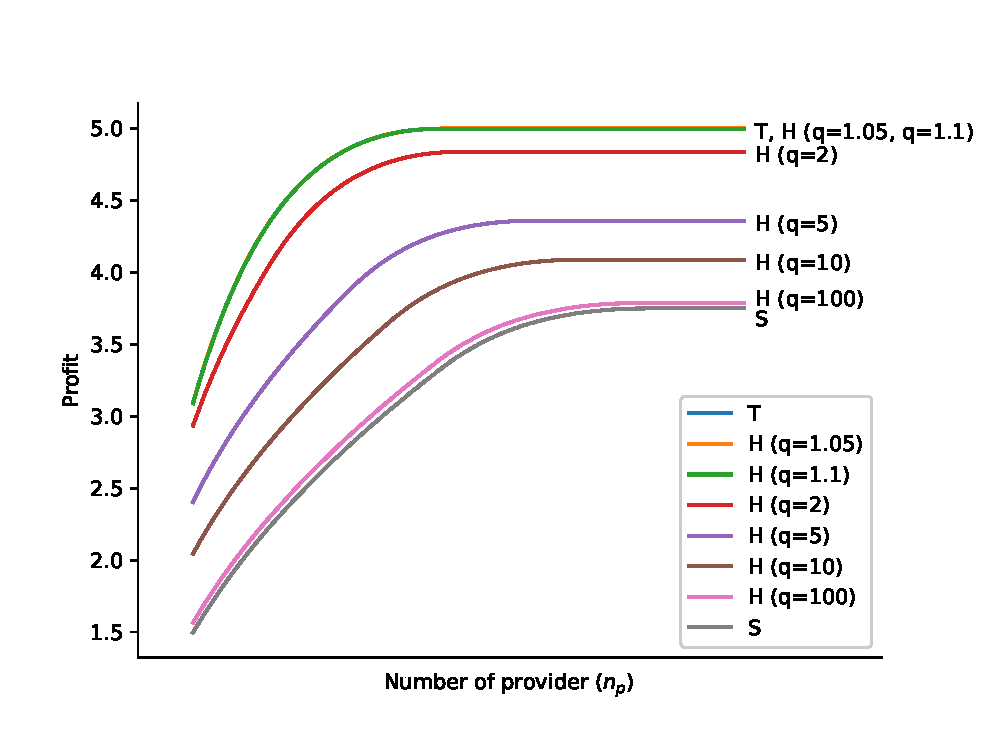
\includegraphics[width=7.5cm]{figure_3rd_final/p2pnum11.eps}}
    \subfigure[Relative profit for case 1]{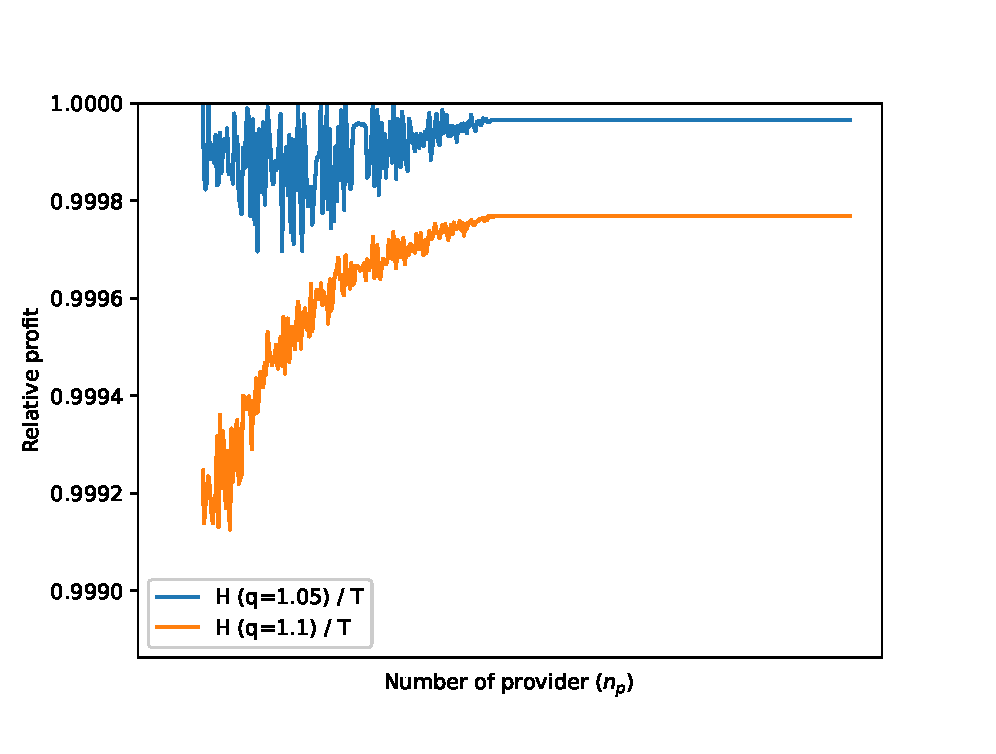
\includegraphics[width=7.5cm]{figure_3rd_final/p2pnum21.eps}}
    \subfigure[Profit for case 2]{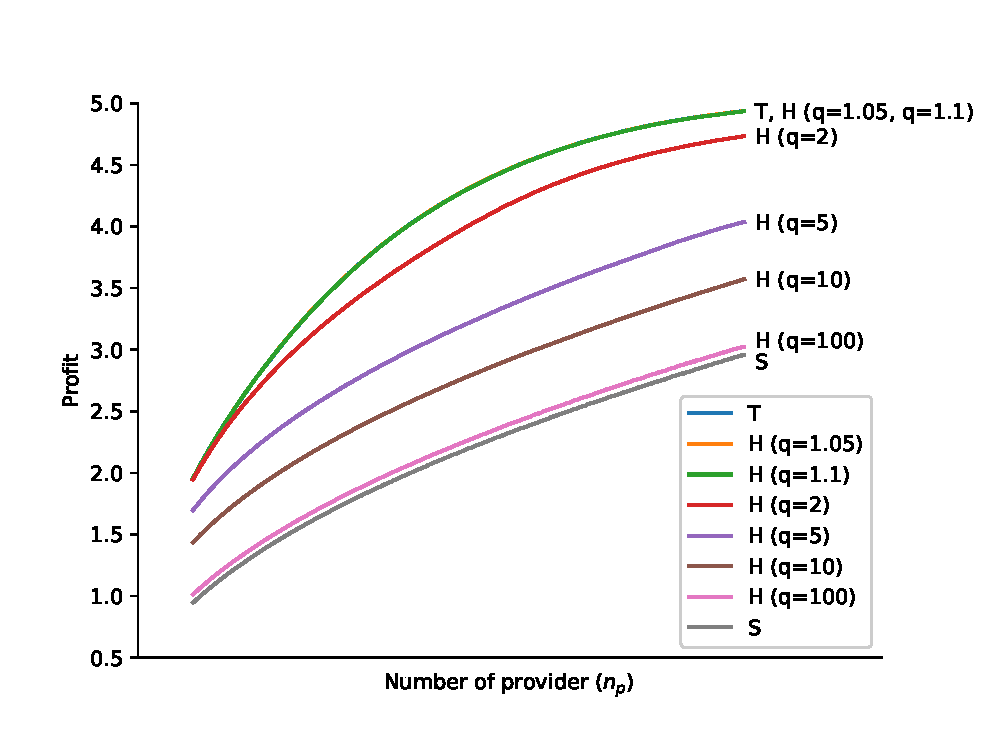
\includegraphics[width=7.5cm]{figure_3rd_final/p2pnum1a.eps}}
    \subfigure[Relative profit for case 2]{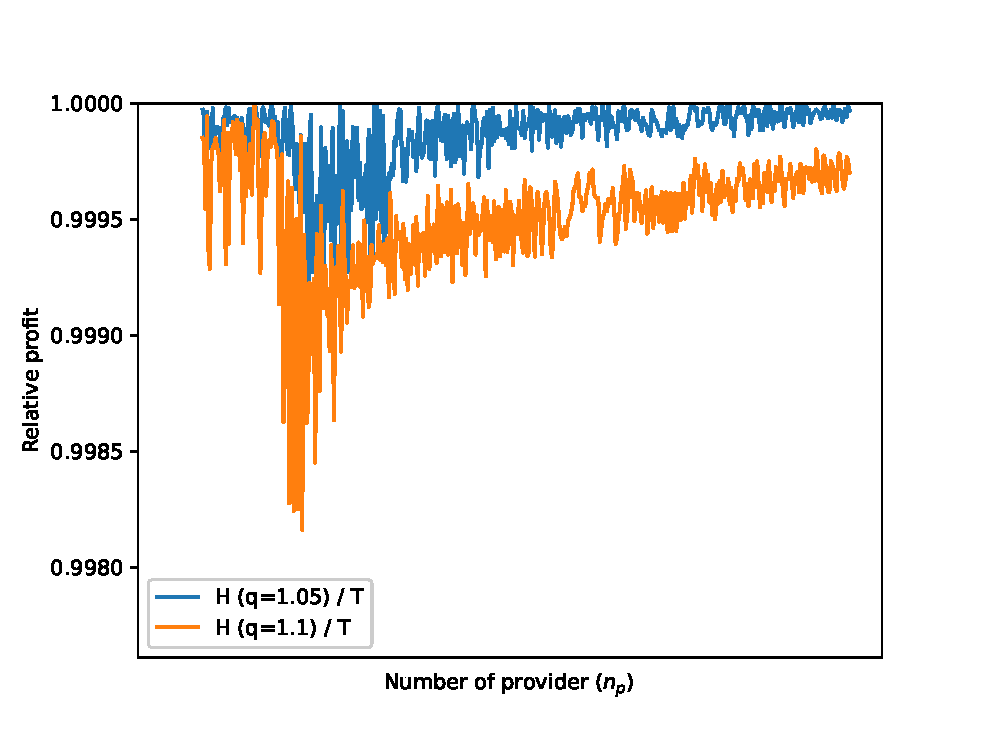
\includegraphics[width=7.5cm]{figure_3rd_final/p2pnum2a.eps}}
    \subfigure[Profit for case 3]{\includegraphics[width=7.5cm]{figure_3rd_final/p2pnum1b.eps}}
    \subfigure[Relative profit for case 3]{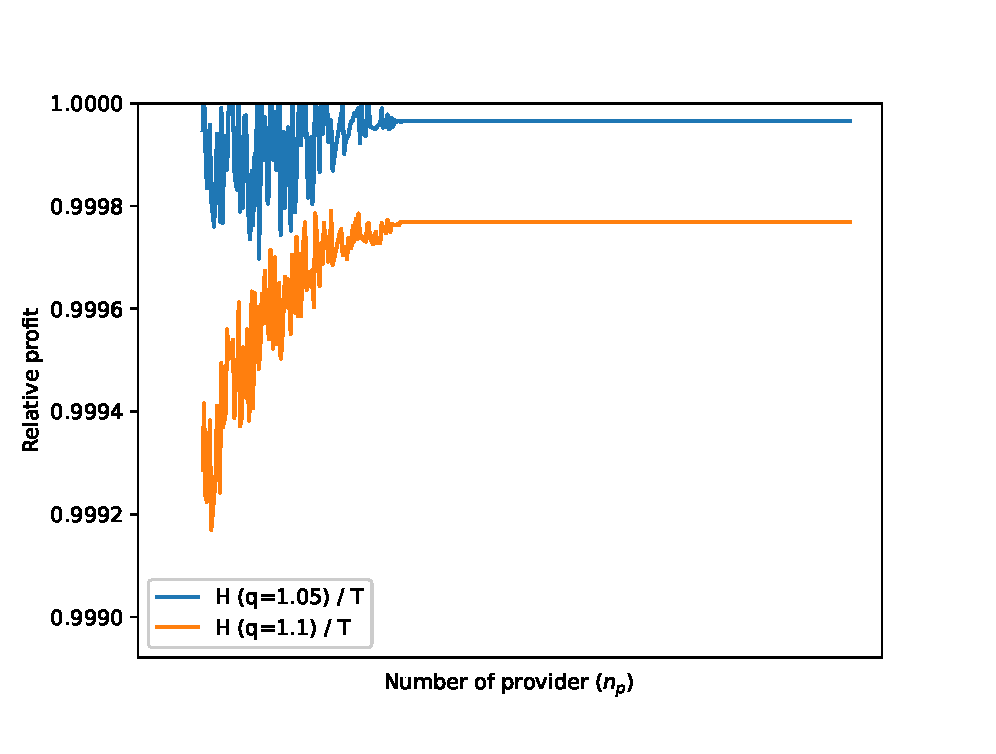
\includegraphics[width=7.5cm]{figure_3rd_final/p2pnum2b.eps}}
    \textbf{\caption{Comparative Profit Analysis
}}
\end{figure}\\

\textbf{2) Welfare Comparison and Implications}

With regard to welfare comparison, our new version provides 1) additional observations from numerical analyses, and 2) the significance of our closed-form solutions for this emerging market.

Regarding the order of the total surplus, we have several results from numerical analyses in Appendix C.2 (Assumptions on Renters). Overall, we observe the followings: 1) a two-part tariff shows a slightly higher total surplus than hybrid pricing when the number of providers is small, and 2) hybrid pricing begins to substantially outperform a two-part tariff since the number of provider reaches $\psi^T$---where subscription-based pricing starts to yield a higher surplus than hybrid pricing. We see such patterns consistently across various conditions.

In this revision, we have supplemented this observation and corresponding insights to Section 6.3, which we were asked to shorten in the last round, as follows:

\textit{``Importantly, we observe from our several numerical analyses that firms can achieve a higher surplus from $Hh$-type hybrid pricing only if either operating costs are extremely low or sufficiently large potential providers (vs. potential renters) exist. Therefore, a two-part tariff is likely the most desirable option, even for the total surplus with a small provider base.'' (page 27)}

Furthermore, this enabled us to supplement our managerial insights for actual services as follows:

\textit{``(...) it is worth noting that Storj introduced a new pricing scheme wherein renters receive a finite amount of free usage volume. Our results suggest that this change can hardly be supported from a profit-seeking perspective in the short term. Also, based on several numerical analyses, we observe that the firm is likely to achieve a higher total surplus only if both the free volume and the potential size of providers are substantial. Therefore, the current choice might not necessarily help its P2P network flourish.'' (page 28)}

Of course, it is valid that the above observation is not mathematically proven and might have some exceptions. We accept this limitation. However, even when we focus only on closed-form solutions, our stylized model still provides valid insights for the following reasons.

Unlike the established sharing economy platforms, such as ride-sharing services (e.g., Uber, Lyft), pricing schemes have not been established and standardized in the immature P2P storage market. In this regard, the complete order of profitability provides meaningful insights for market players. Furthermore, our closed-form solution clearly suggests that subscription-based pricing---which charges zero bandwidth fee on renters---do not necessarily benefit platform participants compared with pricing schemes that charge bandwidth fees under a small provider base. Considering that platforms often prioritize expanding their user base, even at the expense of consecutive years' losses (Bond 2018, Newcomer 2019), this insight can offer clear guidance for decision-making in this emerging industry.

We have added this point in the last paragraph of our paper as follows:

\textit{``(...) it is also worth mentioning that we do not provide the closed-form results of welfare comparison completely. Although our numerical results showed a general tendency that a two-part tariff yields a higher surplus than hybrid pricing with a large free bandwidth allowance, future studies may provide better insights by comparing these pricing schemes more comprehensively.'' (page 29)}

\textbf{References}

Bond, S. (2018) ``Uber aims to be ‘Amazon of transportation’.'' \textit{Financial Times} \url{https://www.ft.com/content/47516aec-d717-11e8-a854-33d6f82e62f8}.

Newcomer, E. (2019) ``Uber revenue growth slows, losses persist as 2019 IPO draws near.'' \textit{Bloomberg} \url{https://www.bloomberg.com/news/articles/2019-02-15/uber-results-show-revenue-growth-slows-amid-persistent-losses}

\newpage
%%%%%%%%%%%%%%%%%%%%%%%%%%%%%%%%%%%%%%%%%%%%%%%%%%%%%%%%%%%%%%%
\textbf{Model:}
\begin{quotation}
{\em
\noindent \textbf{Reviewer 3 (Point 5): }
1. Why are individual providers assigned the same amount of files to store? Shouldn’t providers offer different amounts of storage capacity according to their individual storage costs?
}
\end{quotation}\vspace{-4mm}

Thank you for pointing out this point. We also agree that additional provider heterogeneity can enrich our model and results. Here, let us 1) summarize how the review team and the authors discussed this issue before, 2) describe how this discussion is related to this point, and 3) explain how we have revised our manuscript to complete the final puzzle piece you suggested.

\textbf{1) Summary of previous discussion on provider heterogeneity}

It is worth noting that our model already accounts for three important sources of heterogeneity---two dimensions of renter heterogeneity (download frequency, utility per download) and one dimension of provider heterogeneity (operating costs). In this regard, the review team agreed to adhere to the existing heterogeneity and address the remaining issues based on the current discussion and numerical analyses in the third round review.

Specifically, the review team noted as follows in the second round:

\textit{``Compared to the concern on the unit volume of each renter, perhaps the assumption that each provider supplies unit volume of unused capacity is fine. But the implication is that the provider’s income and cost are both proportional to the volume of capacity supplied. If this is most likely the case in the storage sharing industry, the authors need to explain this point to justify this assumption; otherwise, I wonder whether the authors could relax this assumption, i.e., whether the impacts of a specific pricing scheme on providers with different capacity are different.'' (Reviewer 2's Point A2b)}

In sum, their point was that the assumption that each provider supplies a unit volume of unused capacity requires a condition: the provider’s income
and cost are both proportional to the volume of the capacity provided. Accordingly, we have provided this assumption’s specific justification and potential consequences when this assumption does not hold. To summarize, our assumption is plausible for the following reasons. First, several sources of operating costs are proportional to bandwidth usage, e.g., bandwidth and electricity costs. Second, bandwidth usage is likely proportional to storage volume because P2P storage platforms tend to assign more contracts to high-volume providers. Our revised manuscript was positively evaluated in the third round of review. For clarity, let us mention how we have discussed this point in our manuscript as follows:

\textit{``Second, it is possible that providers have a different cost distribution, which can determine how much they are willing to share storage and bandwidth volumes. Specifically, individuals may have different storage costs, leading to heterogeneous storage capacities in P2P networks. Under such heterogeneous capacities, an alternative form of the provider's operating costs may raise a concern about the validity of our findings. For now, our functional form relies on the assumptions that operating costs are proportional to $\hat{\omega_b}$ (i.e., the expected bandwidth volume for each provider), and that $\hat{\omega_b}$ is proportional to each provider's shared storage capacity. We argue that these assumptions are plausible for the following reasons: 1) many of the major costs, such as Internet bandwidth and electricity costs, are proportional to bandwidth usage, and 2) the platform tends to assign more files and bandwidth services to high-capacity providers than low-capacity ones.}

\textit{So, how would alternative cost forms affect the results? On the one hand, we may consider a convex function, such as quadratic and exponential forms, where operating costs are particularly burdensome for high-capacity providers. In this case, as high-capacity providers bear much higher operating costs and join the platform less, compensating for offering bandwidth services will have a higher impact on the storage capacity. Consequently, the relative benefits of two-part tariff and hybrid pricing (vs. subscription-based pricing) will be greater in this situation. On the other hand, we may also consider a concave function like a square root function. Since high-capacity providers bear relatively less operating burden than they do in the current setup, the platform will attract more providers under the subscription-based pricing. Hence, the profit/surplus gap between the subscription and other pricing schemes will decrease as a result. However, although the magnitudes decline, we expect the differences to remain qualitatively unchanged.''} (pages 25-26)

\textbf{2) How is the previous discussion relevant to your point?}

Assuming that our previous discussion on operating costs is plausible, we would like to revisit your point from that discussion. We can think of two dimensions of provider costs. First, and what we have already considered, is the operating costs of bandwidth provision. Second, we may consider different storage costs that can determine how much storage to share with P2P networks, as you mentioned. To make it clear, we postulate that storage costs refer to a provider's expense to obtain redundant storage space; that is, the higher (lower) costs, the lower (higher) volume a provider will share.

If these two costs are independent---that is, a provider's burden to provide bandwidth is irrelevant to one's storage costs, this is equivalent to the first scenario where operating costs are proportional to bandwidth usage. In this scenario, storage costs can affect the amount of shared storage only; thus, they do not affect our results.

If these costs are associated with each other, the second and third scenarios resemble this situation. On the one hand, if storage costs are negatively related to operating costs for bandwidth provision, high-capacity providers (having low storage costs) bear higher operating costs and join the platform less. Therefore, compensating for offering bandwidth services will have a higher impact on the storage capacity. As a result, the relative benefits of two-part tariff and hybrid pricing (vs. subscription-based pricing) will be amplified, consistent with the second scenario discussed above.

On the other hand, when storage costs are positively related to operating costs for bandwidth provision, high-capacity providers (having low storage costs) bear relatively less operating burden than they do in the current setup, so the platform will attract more providers under subscription-based pricing. Hence, the profit/surplus gap between the subscription and other pricing schemes will decrease, in line with the third scenario above.

\textbf{3) How have we filled the gap between the previous discussion and your point?}

After considering your comment, we have realized that our previous discussion did not address the potential reasons why providers may offer varying amounts of storage space. We admit that missing this point will significantly undermine the philosophy and foundation of our model. To resolve this problem, we have thoroughly revised  the second part of Section 6.2 (Assumptions on Providers) as follows:

\textit{``Second, it is possible that providers have a different cost distribution, which can determine how much they are willing to share storage and bandwidth volumes. Specifically, individuals may have different storage costs, leading to heterogeneous storage capacities in P2P networks. Under such heterogeneous capacities, an alternative form of the provider's operating costs may raise a concern about the validity of our findings.'' (page 26)}

%%%%%%%%%%%%%%%%%%%%%%%%%%%%%%%%%%%%%%%%%%%%%%%%%%%%%%%%%%%%%%%
\begin{quotation}
{\em
\noindent \textbf{Reviewer 3 (Point 6): } 2. In a similar vein, it is a little strange that consumer’s usage of the platform is exogenously given instead of responding to the incentives created by the firm’s pricing scheme.
}
\end{quotation}\vspace{-4mm}

The story continues from our response to \textbf{your point 5}. As mentioned above, our model currently incorporates three important sources of heterogeneity, where two of which are renter characteristics---download frequency and utility per download volume. For your information, let us remind you of our assumption as follows:

\textit{``Based on this assumption, the probability distribution function of the bandwidth usage level can be expressed as $f(\lambda) = \frac{b \lambda_0^b}{\lambda^{b+1}}$, where the minimum bandwidth usage level is denoted by $\lambda_0$. For analytical tractability, we simplify our assumption such that the distribution of bandwidth usage level is characterized by the parameter value of $b = 2$. We also incorporate heterogeneous valuation of a renter's service usage. Specifically, we assume that renter $i$'s utility per unit volume of bandwidth usage (i.e., $u_i$) follows a uniform distribution; that is, $u_i \sim U[0, 1]$. As a result, renter $i$'s total utility obtained from storing files is $\lambda_i u_i$. To focus on the interplay among the platform, providers, and renters, we assume that $\lambda_i$ and $u_i$ are independent.'' (page 10)}

There are several possible ways to extend renter dimensions: 1) different assumptions of the bandwidth usage distributions, 2) relaxing the assumption about the independence of a renter's download utility and the utility per download volume, 3) the heterogeneity of their storage volume, and 4) allowing self-selection of usage amounts. Among them, the first three concerns were raised by the review team. Due to analytical tractability, we relied on numerical analyses to observe whether our insights remained consistent in different assumptions and conditions (please refer to Section 6.3). Our results were positively considered and not mentioned further in the last round.

Regarding the last point, we admit that our analyses did not account for the self-selection of usage amounts. It is worth noting that while the extant literature on cloud services often considered a usage distribution of potential customers not affected by pricing schemes (e.g., Chen et al. 2019), this does not imply that cloud users cannot determine their usage amounts flexibly in reality. Moreover, although relaxing the independence assumption between a renter's download utility and the utility per download volume can enhance the self-selection process of \textit{adopting} the platform, it still does not address the self-selection of usage amount \textit{within each platform adopter}. Therefore, if such a limitation is not discussed, journal readers might perceive that this research ignored this important aspect without consideration. To avoid overlooking this important aspect, we have revised our manuscript as follows:

\textit{``Moreover, our model does not consider the possibility that renters may change their usage levels depending on pricing schemes, which can provide a valuable direction for future research.'' (page 29)}

\textbf{References}

Chen, Shi, Hau Lee, and Kamran Moinzadeh. "Pricing schemes in cloud computing: Utilization‐based vs. reservation‐based." \textit{Production and Operations Management} 28.1 (2019): 82-102.

\end{document} 